\documentclass[10pt,conference,compsocconf]{IEEEtran}

\usepackage{hyperref}
\usepackage{graphicx}	% For figure environment
\usepackage{amsmath}
\usepackage{amssymb}
\usepackage{float}
\usepackage{url}
\newcommand{\beginsupplement}{%
	\setcounter{table}{0}
	\renewcommand{\thetable}{S\arabic{table}}%
	\setcounter{figure}{0}
	\renewcommand{\thefigure}{S\arabic{figure}}%
}

\begin{document}
\title{CS-433 Machine Learning Project 2}

\author{
  Matthias Minder, Zora Oswald, Silvan Stettler\\
}

\maketitle

\begin{abstract}
Abstract...
\end{abstract}

\section*{Introduction} 
The recently developed method of single cell RNA sequencing (scRNA-seq) allows to measure the amount of RNA from a specific gene at the single cell resolution. This gives valuable insight into the properties and cellular function of single cells in a whole population of cells. High throughput methods allow to analyze thousands of cells simultaneously. scRNA-seq results in so-called read-count matrices (RCMs) which indicate the expression level of a given gene in a given cell.
\par 
The emergence of scRNA-seq has led to the discovery of many new cell populations based on their gene expression profile. The question thus naturally arises whether it would be possible to predict cell types using a machine learning approach. To this effect, classifiers can be trained on various publicly available data sets to infer cell types on a new data set. Of special interest is the detection and \textit{de novo} discovery of stem cells in tissues for which no stem cell population has been characterized. It is still unknown whether there exist specific biomarkers for multipotent stem cells allowing to identify them across tissues, which makes this problem attractive to solve. 
\par
However, several challenges are associated with working with scRNA-seq data. The three most predominant issues are the following: Differences in protocols and procedures between give rise to batch effects, leading to substantial overall differences between datasets of different sources. Secondly, cell-type annotation is based on clusters of the dataset itself and thus depends on the  analysis and interpretation of the data. This may lead to biases when basing analysis on the annotated clusters. Thirdly, the obtained data is perturbed by so called drop-out events, where the read-counts for a given gene is measured to be zero, even if there were a signal. The result is that RCMs are very sparse. 
\par
Additional issues arise from a machine learning perspective: Since the expression of different genes can be functionally related or controlled by the same transcriptional regulatory program, some features are highly correlated. However, due to the noisy nature of the data, identifying highly correlated features is difficult. The scRNA-seq data can thus be thought of as being on a sub-dimensional manifold. An accurate representation of this manifold is key for obtaining stable results that generalize well to other data sets in order to overcome batch-effects. Moreover, a good such representation also reduces the impact of drop-outs: If several genes are simultaneously expressed for a given biological process, and a subset of these aren't detected due to drop-outs, the other genes could correct this. Naturally, such an approach doesn't work when the drop-out rate is too high. Overall, this nature of scRNA-data suggests that the application of dimensionality reduction prior to method training will yield results that perform better on independent test data.
\par
Within this report, we compare the prediction performance of different stem cell classifiers based on an independent test set in order to finally determine the best-performing classifier. The presented classifiers are based on different, well-established machine learning methods and were trained on data subjected to different data transformations and dimensionality reduction techniques.

\section*{Methods}
\subsection{Experimental Setup}
For the entire analysis, 17 publicly available datasets were used [CITATION]. These data sets were split into three sets, train set (eleven data sets), test set (three data sets) and the generalization train set (four data sets). Two types of classifiers were trained, which will be called basic and nested classifiers. The basic classifiers were trained on the training set, and their predictive performance was assessed in terms of accuracy on the test set. The nested classifiers were trained as follows: Using the basic classifiers, predictions were generated for the data in the generalization train set. Then, the resulting predictions by all basic classifiers were used as training set for a second classifier, whose performance was assessed on the test set. By constructing the two-layer nested classifiers, we hoped to be able to obtain a final model which is less prone to batch effects. 
Different basic classifiers were trained on a total of eight data transformations described below, six of which are network-based. 

\subsection{Dataset Preparation}
Cell type annotation was based on the clustering done in the original papers. All three sets consist only of cells which were determined as being stem or non-stem in order to avoid introducing a bias into the model. Notably, progenitors, endothelial and fibroblast cells were excluded from the analysis. For the train set, the cells were down-sampled to be of equal proportions from the three different germ layers, and within each germ layer 50\% stem and 50\% non-stem. This was chosen in order to avoid introducing a tissue-specific bias in determining stem-ness. 
\par
Since different datasets measure the expression of different genes, one has to choose which genes to use for the analysis in order to be able to fuse different datasets. The genes retained for our analysis were selected as follows: For all eleven sets within our train set, we determined whether they contained stem cells, non-stem cells or both. Then, the genes represented in all sets with stem-cells was combined with the genes represented in all sets containing non-stem cells. The reasoning behind this was that in this way, genes that are only expressed in one category of cells, stem or non-stem, are retained while minimizing the number of genes with missing values. This resulted in 13'587 genes retained for further analysis.
\par
For datasets in which a necessary gene isn't represented, we set the gene expression to zero. This is based on the heuristic that such genes are lowly expressed in these datasets, as otherwise they would have been sufficiently measured to be retained in the final dataset. 
\par
After retaining only the necessary genes and filling missing values with zero, we normalized the expression values to transcripts per million before transforming the values with $ln(1+x)$. This is standard procedure for scRNA-seq data. All subsequent transformations and training steps was based on data in this format. 

\subsection{Dimensionality Reductions}
The dimensionality of the data was reduced using conventional Principal Component Analysis (PCA) and two methods based on graph signal processing (GSP) on a graph constructed using a protein interaction network.
\par
Taking into account external information about the underlying structure is another way to reduce the influence of set specific batch effects. To this effect, we included a protein interaction network, which we then use as topology to process the expression signal. Protein interaction networks are representations of the physical and biochemical interaction between proteins in an organism. By linking proteins with the genes encoding them, a protein interaction network can be converted to a gene network. 
\par
In the protein interaction network used here, the weight of the edges between individual proteins, which form the nodes, are a measure of how confidently an interaction can be judged to be true. The protein interaction data that was used is available in the STRING database (\url{www.string-db.org}) \cite{Szklarczyk2016}. By replacing each protein in the network with the gene that encodes it, a gene network can be created. The genome along with the corresponding expressed proteins for \textit{mus musculus} are available in the Ensembl database (\url{www.ensembl.org}) \cite{Zerbino2017}. For the creation of our network, only the proteins that could be associated to an expressing gene were kept.
Self-loops that resulted from genes whose expression produces multiple proteins and isolated nodes (no link to another node) were removed, yielding a network with 20330 genes forming nodes that are connected by 11'856'336 edges. It has to be mentioned that the gene network is constructed based on the entire dataset that was available from the sources mentioned above. Contrary to the analysed data, the scope of the network does not limit itself to the genes found in a particular type of cells, such as tissue.  \\
The process of creating the gene network is schematically shown in \ref{fig:network_creation}.
\begin{figure}
	\centering
	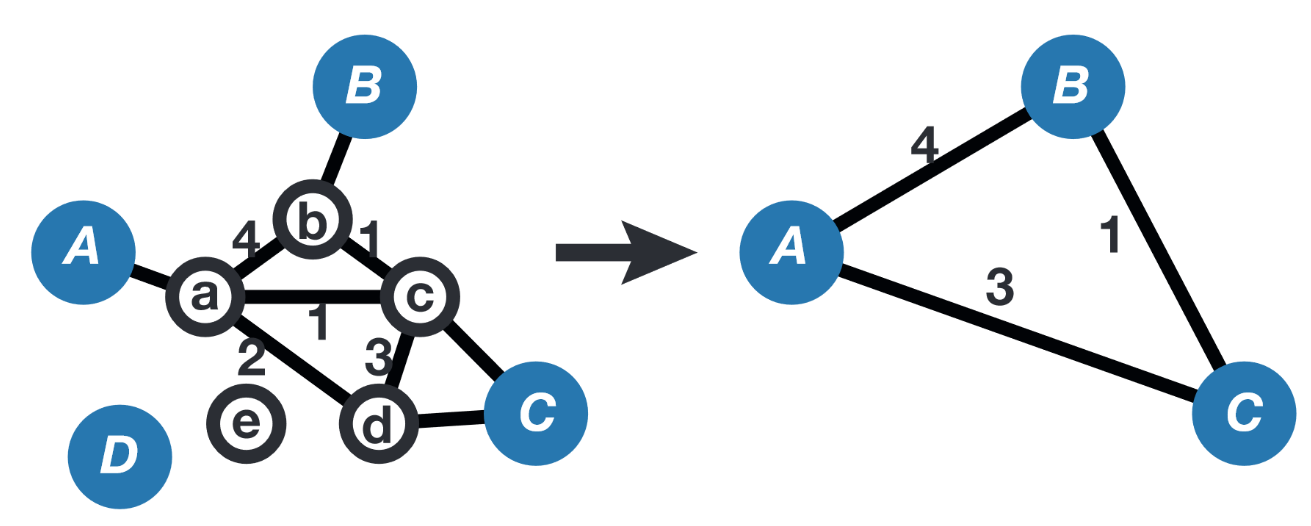
\includegraphics[width=0.45\textwidth]{network.png}
	\label{fig:network_creation}
	\caption{Schematic of network creation}
\end{figure}
In TODO the genes \textit{A, B, C, D} in blue are associated with the proteins that their expression produces. It is possible that the expression of a gene can result in multiple proteins, such as the gene \textbf{C} that codes for proteins \textit{c} and \textit{d}. The nodes in the original protein interaction network are then replaced with the gene that is responsible for their creation. In the case of the genes \textit{A} and \textit{C} in Figure \ref{fig:network_creation}, this yields two edges between the same genes. Thus, such genes are linked with only one edge with a weight equal to the sum of all the incident edge weights to the concerned proteins. The self-loops that might occur due to two linked proteins being expressed by the same gene such as \textit{c} and \textit{d} in the above example are removed. Proteins that could not be associated to a gene or vice versa are also removed from the network.
The original score $s_{ij}$ of a link between nodes $i$ and $j$ was used to compute an equivalent distance, where high scores result in a short distance. Subsequently, new link weights $W_{ij}$ were set using a Gaussian kernel.

\begin{align}
d_{ij} &= \frac{1}{s_{ij}} \\
W_{ij} &= exp (- \frac{d_{ij}^2}{2 \sigma^2})
\end{align}
\par

The scRNA-sec data can be transformed into a graph signal by assigning the count of expressed genes to the corresponding gene in the network, yielding a signal $\boldsymbol{x} \in \mathbb{R}^N$, where $N$ is the total number of nodes. Genes whose expression was not present as a feature in the scRNA-sec data are assigned 0. \\
After mapping the data onto the resulting graph, graph signal processing (GSP) can be leveraged to find a lower-dimensional manifold that embeds the original data, based purely on the interaction of the protein expression of the genes. The two methods that were applied take advantage of the fact that the eigendecomposition of the $N x N$ graph Laplacian matrix $\boldsymbol{L} = \boldsymbol{U\Lambda U}^T$ forms the equivalent of a Fourier basis on a graph, where $\boldsymbol{U}$ are the $N$ Fourier basis vectors and the $N$ eigenvalues $\boldsymbol{\Lambda}$ represent the corresponding frequencies.
 \par
Graph sampling (GS) aims to find nodes where signal energy is the most concentrated for frequencies in the range $(f_{min}, f_{max})$. The \textit{local graph coherence} at node $i$ of order $k$ is defined as the square of the $i$-th entry of the $k$-th eigenvector $u_{ik}$ of the Laplacian, which is a measure for how localized the first $k$ Fourier modes are on node $i$ \cite{Puy2018}. By choosing the first $K$ indices $i$ that maximize $\Sigma_{k=f_{min}}^{f_{max}} u_{ik}^2$, the data can be reduced to the $K$ genes whose read-count information has the most value based on their location in the network for the chosen frequency range. In particular, we applied the GS algorithm for only low frequencies (below N/2) and only high frequencies (above N/2). 
\par
The idea behind graph frequency sampling (GFS) is essentially to transform the data into the spectral domain and retain components above or below a certain frequency. The Graph Fourier Transform (GFT) and its inverse are given by
\begin{align*}\label{equ:GFT}
\boldsymbol{\hat{x}} &= \boldsymbol{U}^T \boldsymbol{x}\\
\boldsymbol{x} &= \boldsymbol{U} \boldsymbol{\hat{x}}
\end{align*} 
\par
In our GFS algorithm, the graph signal is projected only onto the $K$ eigenvectors associated to eigenvalues below or above a cut-off frequency, resulting in a $K$-dimensional signal $\boldsymbol{\hat{x}_{GFS}}$. For example, choosing the $K$ lowest frequencies,
\begin{equation}
\boldsymbol{\hat{x}_{GFS}} = \boldsymbol{U}[0:K]^T \boldsymbol{x}.
\end{equation} 
\par
We used the the $K$ lowest and highest frequencies to transform the original data. GFS potentially mitigates issues due to batch effects that might appear as a low-frequency component in the graph signal. Similarly, the presence of drop-outs might manifest itself as a high-frequency component and thus be filtered when considering only low-frequency eigenvectors.\\
\par
The GFT was also used to implement a simple low or pass rectangle filter of the data using the network. After transforming the data into a graph signal as described previously, the GFT is computed (Equation \ref{equ:GFT}). The components of the resulting spectrum that are above or below a cut-off frequency are set to zero. Subsequently, the inverse GFT given by is applied to obtain a filtered version of the original signal. While this process does not reduce the dimensionality of the data, it could provide insight on validity of the network creation process and reduce noise.
\par
In summary, 8 different methods are used to transform the data and reduce dimensionality: PCA, Graph sampling (LF and HF), Graph frequency sampling (LF and HF), Graph filtering (LF and HF) and a nested method that combines all the above.

\subsection{Machine Learning Methods}
Within this project, we applied four different types of classifiers: Logistic regression, random forest, neural net and XGboost.
\par

The neural net consists of six fully connected layers used as classifier into the two classes not stem cell and stem cell. The probabilities are then computed using a softmax classifier. The net was trained with stochastic gradient descent on the cross entropy loss in ten epochs. In order to find the best learning rate and regularization constant, validation on part of the training set was conducted for different parameters during one epoch each. The best learning rate and weight decay were retained after two refinements. During the training of the neural net, a learning weight decay was used to avoid oscillating across the optimum.


\section*{Results}

The accuracies of the basic classifiers on the training set are summarized in Figure \ref{fig:train_acc} below.
\begin{figure}
	\centering
	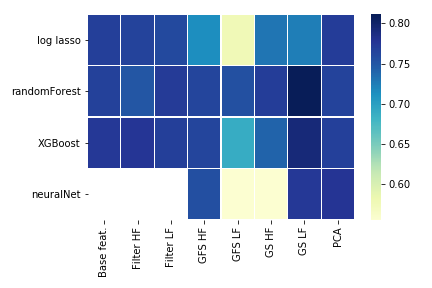
\includegraphics[width=0.45\textwidth]{train_accuracy.png}
	\label{fig:train_acc}
	\caption{Accuracy on training set of the basic classifiers}
\end{figure}
The following accuracies were obtained with all classifiers, including the nested classifier that was previously trained on the generalized training set.
\begin{figure}
	\centering
	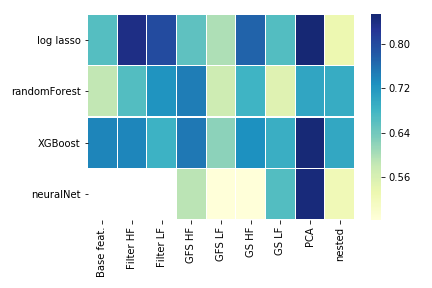
\includegraphics[width=0.45\textwidth]{test_accuracy.png}
	\label{fig:test_acc}
	\caption{Accuracy on the test set of all classifiers }
\end{figure}
On the figures above we can observe that the impact of the choice data transformation is significant. Overall, the best results were achieved using conventional PCA. Accuracies with PCA on the test were similar for all four classifier with a maximum of 93.4\% with log lasso and in all cases better than the baseline model.
The accuracy of the predictions when using the network based GS and GFS transformations has a stronger dependence on classifier type and achieves lower accuracies overall than PCA. However, in certain cases, accuracies well superior to the baseline model with the same classifier were obtained, for example with GS HF and log lasso or GFS HF and random forest. In general, the results suggest that the performance is heavily dependent on the choice of classifier when using a network-based transformation, contrary to PCA.   

\par  
Predictions with graph-filtered data without dimensionality reduction on the test set are slightly more accurate than the baseline model, hence indicating that using a gene network based on protein interactions can be a valid preprocessing method.

\section*{Conclusion}

%%% Bibliography
\bibliographystyle{IEEEtran}
\bibliography{literature-project2}

\beginsupplement

\begin{table}[H]
	\centering
	\begin{tabular}{rrrrrrrr}
\hline
  77.0 &  76.7 &  76.1 & 71.4 & 57.6 & 73.1 & 72.4 & 77.2 \\
  76.8 &  75.0 &  77.3 & 76.4 & 75.5 & 77.1 & 81.1 & 76.7 \\
  77.5 &  77.7 &  77.0 & 76.4 & 68.9 & 74.2 & 79.3 & 76.9 \\
 nan   & nan   & nan   & 75.7 & 55.5 & 55.5 & 77.5 & 77.7 \\
\hline
\end{tabular}
	\caption{Accuracies on train set, raw data}
\end{table}

\begin{table}[H]
	\centering
	\begin{tabular}{rrrrrrrrr}
\hline
  66.4 &  83.8 &  80.0 & 65.6 & 59.9 & 77.2 & 66.4 & 85.4 & 53.4 \\
  58.5 &  66.5 &  72.6 & 74.9 & 57.4 & 68.2 & 55.2 & 70.2 & 69.4 \\
  73.9 &  73.8 &  68.5 & 75.3 & 62.2 & 72.9 & 69.0 & 85.1 & 70.0 \\
 nan   & nan   & nan   & 59.1 & 48.3 & 48.3 & 66.4 & 84.7 & 52.6 \\
\hline
\end{tabular}
	\caption{Accuracies on test set, raw data}
\end{table}

\end{document}
